Use the FFT in $N$ points to calculate the first 20 Taylor series coefficients of 
$f(z) = \log(1 + \frac12z)$. What is the asymptotic convergence factor as $N\rightarrow\infty$? 
Can you explain this number?\\

\begin{solution}\renewcommand{\qedsymbol}{}\ \\
    To get the first 20 coefficients of the Talor series expansion, we need to spectrally differentiate
    using the FFT. Now, we will consider the series centered about $x=0$. By this, we know that the
    first coefficient is given by $a_0=f(0)=0$. As such, we only need the first nineteen derivatives.
    Using differential calculus, we have that the $nth$ derivative of $f$ is given by:

    $$f^{(n)}=\frac{(-1)^{n+1}}{(x+2)^n}$$

    Hence, the $nth$ coefficient of the desired Taylor series is given by

    $$a_n=\frac{1}{n!}(\frac{(-1)^{n+1}}{2^n})$$

    The code below gives us the following coefficients for $N=30$ using the FFT function:

    $$a_1=0.5000\;\; a_2=-0.1250\;\; a_3=0.04167\;\; a_4=-0.01563\;\; a_5=0.00625$$

    $$a_6=-0.002604\;\; a_7=0.001116\;\; a_8=-4.8828\times10^{-4}\;\; a_9=2.1701\times10^{-4}\;\;
    a_{10}=-9.7656\times10^{-5}$$

    $$a_{11}=4.4389\times10^{-5}\;\; a_{12}=-2.0345\times10^{-5}\;\; a_{13}=9.3900\times10^{-6}\;\;
    a_{14}=-4.3597\times10^{-6}$$
    
    $$a_{15}=2.0345\times10^{-6}\;\; a_{16}=-9.5367\times10^{-7}\;\; a_{17}=4.4879\times10^{-7}\;\;
    a_{18}=-2.1193\times10^{-7}$$

    $$a_{19}=1.0039\times10^{-7}$$

    From here, we get the following plot of the error between the computed coefficients and the actual
    coefficients.

    \begin{center}
        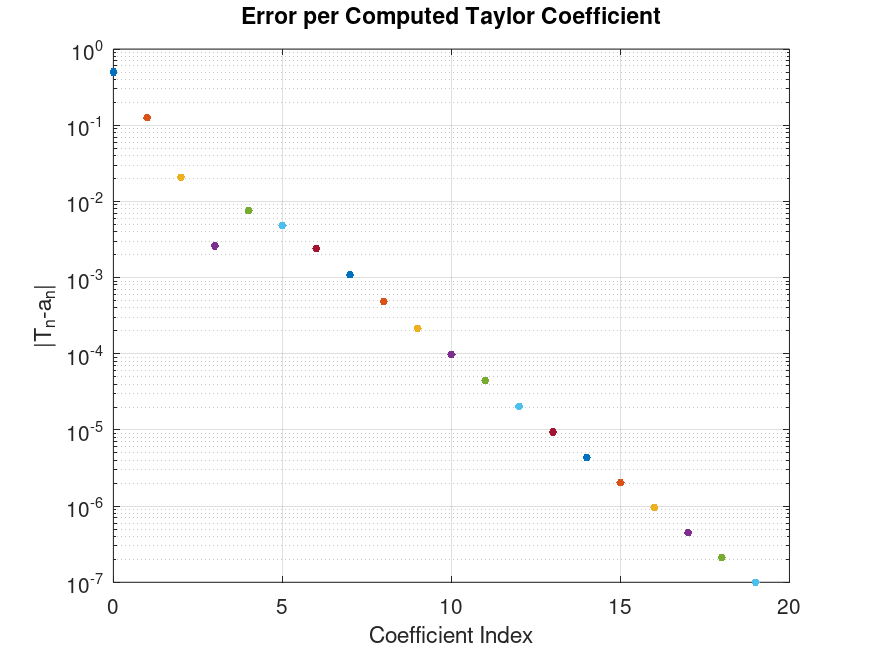
\includegraphics[scale=0.45]{problem12_7.PNG}
    \end{center}

    Since this is a semilog plot with respect to y, we see that the error is exponentially convergent
    as $N$ tends towards infinity.

\end{solution}

\newpage
\lstinputlisting{problem12_7.m}
\newpage